\chapter{Experimentos e resultados}
\label{CAP5}

Neste capítulo são apresentados os experimentos realizados no ambiente montado, como os testes foram realizados e quais considerações foram adotadas. Em segurança da informção é muito importante saber se defender de um ataque, ou saber que está sendo atacado, porém, para identificar um ataque ou saber se defender dele, é necessário saber realizar um ataque.

Tendo isso mente, foram realizados três tentativas de ataques diferentes, nos quais são explicados nas seções sequintes. As boas práticas de segurança da informação ou segurança dos dados vão muito além de senhas e sistemas com \textit{firewalls}, a segurança dos dados consiste de uma política bem elaborada pelos responsáveis e com todos da equipe respeitando essa política.

Os experimentos seguem as boas práticas de um \textit{pentest}, ou seja, seguindo as etapas de \textit{scanner}, exploração, e entre outras etapas já citadas. Os experimentos seguiram a sequinte sequência: \textit{scanner}, recolhimento de informações, ataque e por fim boas práticas de segurança para minimizar os danos ou dificultar a ação dos \textit{hackers}, essas boas práticas de segurança são dicas para ser seguidas e com isso evitar maiores transtornos.

\section{Cenário I}

Neste primeiro cenário a ideia principal consiste em testar uma das funcionalidades do \textit{framework} Apache Hadoop, que é a tolerância a falhas, ou seja, o ataque será direcionado a um nó do cluster, com o intuito de sobrecarregá-lo, com isso, segundo a literatura do Apache Hadoop, ela diz que o \textit{framework} é tolerante a falhas, e nestes momentos ele sabe se comportar, em caso de um nó sobrecarregado ele consegue distribuir as suas tarefas para os demais nós do cluster, então considerando essa informação, foi sugerido um ataque de negação de serviço, ou seja, um DoS, que consiste em apenas uma máquina enviando pacotes de requisições para o nó, na tentativa de derrubá-lo ou sobrecarregá-lo.

Como explicado anteriormente, a vítima é um nó do cluster, enquanto que o atacante é uma máquina com o sistema operacional Kali Linux. Ao realizar o \textit{scanner} da rede com o comando "nmap -T4 -A -v 10.0.0.0/24", obteve-se os resultados apresentados nas figuras \ref{Fig:Scaneando a rede} e \ref{Fig:Scaneando a rede mais completo}.

Os resultados apresentados nas figuras \ref{Fig:Scaneando a rede} e \ref{Fig:Scaneando a rede mais completo}, ilustram muitas informações a respeito das vítimas. Este \textit{scanner} permite identificar qual o sistema operacional, qual a versão do \textit{kernel}, quais serviços estão rodando, quais as portas que estão abertas e qual o nível de dificuldade que o atacante irá encontrar ao tentar quebrar a segurança. Da figura \ref{Fig:Scaneando a rede mais completo} pode-se extrair que o sistema operacional usado pelo cluster é o Ubuntu Linux 3.x ou 4.x e o \textit{kernel} 3.x ou 4.x.

Como qualquer sistema que esteja na internet está sujeito a um ataque de negação de serviço e tendo em vista, que a proposta deste primeiro ataque é verificar como o cluster Hadoop se comporta quando está sofrendo uma sobrecarga, tem-se então o cenário ideal para realizar um DoS.

O \textit{software} utilizado para realizar o ataque foi o HPING, que é um \textit{software} muito poderoso quando se trata de ataque de DoS, sendo assim, ao acessar o kali linux (máquina atacante), do terminal foram executados os seguintes comandos: "hping3 10.0.0.2 -p 80 -S --faster --rand-source". Com esse comando o atacante estará enviando 10 pacotes por segundo para a vítima com o IP 10.0.0.2, utilizando a porta 80. Esses pacotes enviados funcionam da seguinte forma:

\begin{enumerate}
	\item O cliente envia uma solicitação de conexão, com um pacote TCP sem dados, possuindo o flag de SYN ligado e os demais desligados. Por causa da presença do flag de SYN, este pacote é conhecido como pacote SYN.
	
	\item Se o servidor quiser e puder atender, devolve um pacote ao cliente ainda sem dados, com os flags de SYN e de ACK ligados. Está segunda etapa é conhecida como SYN/ACK.
	
	\item Se o cliente ainda quiser manter a conexão, devolve ao servidor um terceiro pacote sem dados, apenas com o flag de ACK ligado (SYN desligado).
\end{enumerate}

Somente após a terceira etapa é que os dados podem ser trocados. Quando o cliente realiza uma requisição ao servidor, o servidor aloca memória para a requisição do cliente e para a resposta, isso é chamado de \textit{handshake} de três vias, ou seja, o \textit{3way handshake}. O não cumprimento da segunda etapa por parte do cliente consome a memória alocada do servidor, sendo assim, muitos pacotes enviados o servidor irá ficar sobrecarregado e não conseguirá responder.

Os ataques foram realizados da seguinte forma: Primeiro foi executada uma tarefa de exemplo do Hadoop, dai mediu-se o tempo gasto pelo Hadoop para concluir essa tarefa, sem executar nenhum ataque. Após isso, iniciou-se os ataques com o tempo sendo cronometrado e executando a mesma tarefa, a tabela \ref{dadosDoDDOS} demonstra os dados avaliados.


\begin{figure}[htbp!] \begin{center}
% fbox faz uma borda ao redor do seu argumento
\fbox{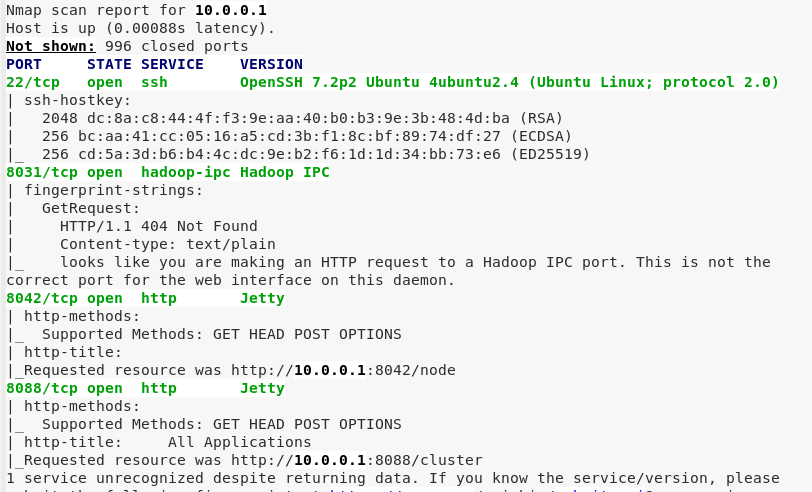
\includegraphics[width=0.80\linewidth]{figures/scaneamentoCompleto01}}
\caption{Scaneando a rede}
\small{Fonte - (próprio autor, 2018)}
\label{Fig:Scaneando a rede}
\end{center} \end{figure}

\begin{figure}[htbp!] \begin{center}
% fbox faz uma borda ao redor do seu argumento
\fbox{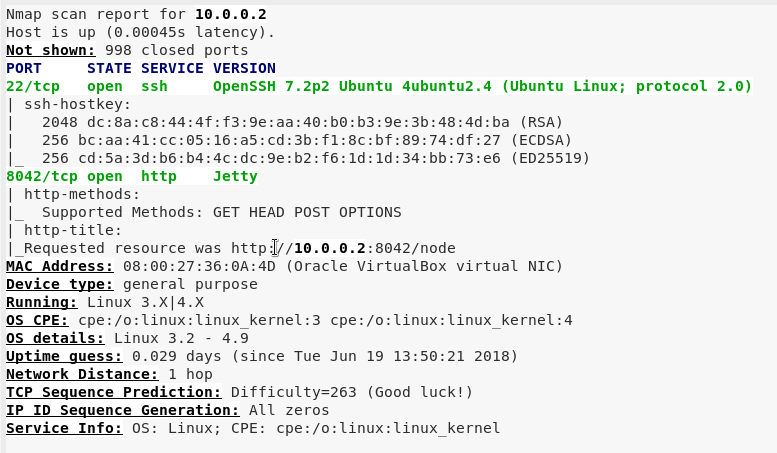
\includegraphics[width=0.80\linewidth]{figures/scaneamentoCompleto02}}
\caption{Scaneando a rede mais completo}
\small{Fonte - (próprio autor, 2018)}
\label{Fig:Scaneando a rede mais completo}
\end{center} \end{figure}

\newpage

% ######## init table ########
\begin{table}[h]
 \centering
% distancia entre a linha e o texto
 {\renewcommand\arraystretch{1.25}
 \caption{Dados do ataque DoS}
 \label{dadosDoDDOS}
 \begin{tabular}{ l l l }
  \cline{1-1}\cline{2-2}\cline{3-3}  
    \multicolumn{1}{|p{3.150cm}|}{\textbf{Duração do ataque (minutos)} \centering } &
    \multicolumn{1}{p{4.500cm}|}{\textbf{Tempo de execução da tarefa hadoop (segundos)} \centering } &
    \multicolumn{1}{p{2.350cm}|}{\textbf{Quantidade de pacotes enviados} \centering }
  \\  
  \cline{1-1}\cline{2-2}\cline{3-3}  
    \multicolumn{1}{|p{3.150cm}|}{0 \centering } &
    \multicolumn{1}{p{4.500cm}|}{147,892 \centering } &
    \multicolumn{1}{p{2.350cm}|}{0 \centering }
  \\  
  \cline{1-1}\cline{2-2}\cline{3-3}  
    \multicolumn{1}{|p{3.150cm}|}{5 \centering } &
    \multicolumn{1}{p{4.500cm}|}{178,673 \centering } &
    \multicolumn{1}{p{2.350cm}|}{8234110 \centering }
  \\  
  \cline{1-1}\cline{2-2}\cline{3-3}  
    \multicolumn{1}{|p{3.150cm}|}{10 \centering } &
    \multicolumn{1}{p{4.500cm}|}{180,754 \centering } &
    \multicolumn{1}{p{2.350cm}|}{13546404 \centering }
  \\  
  \cline{1-1}\cline{2-2}\cline{3-3}  
    \multicolumn{1}{|p{3.150cm}|}{15 \centering } &
    \multicolumn{1}{p{4.500cm}|}{189,357 \centering } &
    \multicolumn{1}{p{2.350cm}|}{20157836 \centering }
  \\
  \cline{1-1}\cline{2-2}\cline{3-3}  
    \multicolumn{1}{|p{3.150cm}|}{20 \centering } &
    \multicolumn{1}{p{4.500cm}|}{212,469 \centering } &
    \multicolumn{1}{p{2.350cm}|}{23817843 \centering }
    \\
  \hline

 \end{tabular} }
\end{table}


\begin{figure}[htbp!] \begin{center}
% fbox faz uma borda ao redor do seu argumento
\fbox{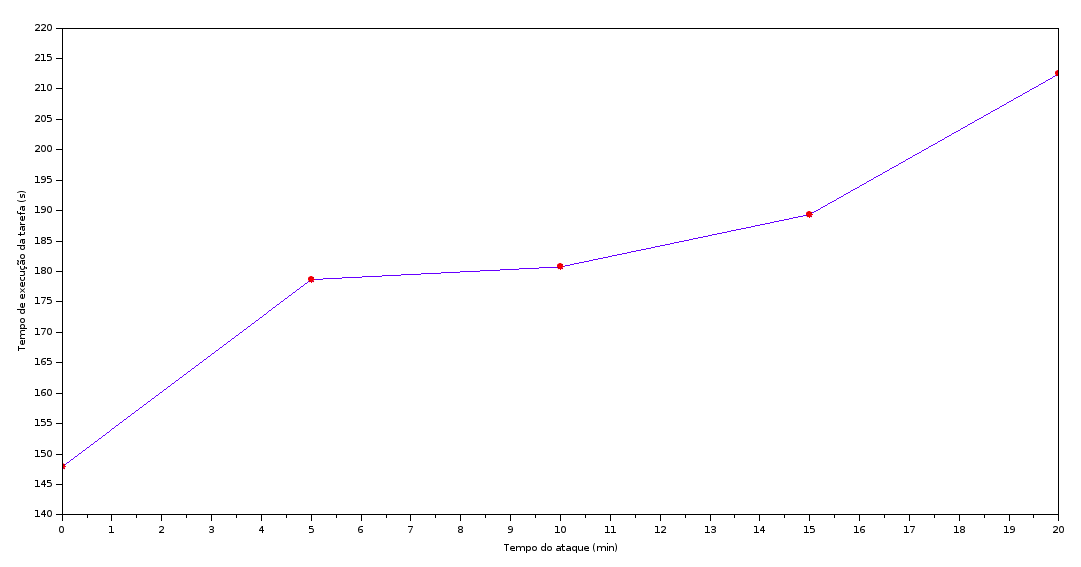
\includegraphics[width=1.0\linewidth]{figures/graficoDOS}}
\caption{Gráfico do DoS}
\small{Fonte - (próprio autor, 2018)}
\label{Fig:grafico do dos}
\end{center} \end{figure}

Levando em consideração que esse ataque é composto por apenas uma máquina e que existem algumas limitações de \textit{hardware}, tendo isso em mente, pode-se perceber que houve uma pertubação no meio fazendo com que o \textit{framework} demorasse mais tempo para concluir sua tarefa. De acordo com os dados percebe-se que se existissem mais máquinas enviando pacotes para um determinado nó do cluster ele ficaria altamente sobrecarregado, sendo assim as tarefas do cluster demorariam mais tempo para serem executadas, ou seja, quanto mais tempo o atacante passou enviando pacotes, mais tempo a tarefa demorou a ser concluída, isso pode ser uma dor de cabeça para empresas que precisam de resultado rápido para tomar decisões.

A figura \ref{Fig:grafico do dos} exibe uma função quase linear, ou seja, a medida que o ataque de negação de serviço demora, aumenta também o tempo de execução da tarefa pelo Hadoop, sem contar que durante a executação da tarefa mediante ataque foi percebido que o \textit{framework} Hadoop teve que 'matar' alguns dos seus processos para poder executar a tarefa proposta, liberando recursos para finalizar o \textit{Job}, enquanto estava sob ataques DoS.

Levando em consideração que esse ataque é realizado em pequena escala, ou seja, apenas de um host para outro determinado host e em um ambiente controlado. Pensando em um ambiente de produção de uma grande empresa e com milhares de hosts, esse ataque poderia causar sérios danos a infraestrutura da empresa escolhida.

\subsubsection{Boas práticas de segurança}

Sabendo que nenhum sistema está completamente protegido e que eles podem eventualmente sofrer algumas falhas, as boas práticas de segurança em ambiente Hadoop propõem a utilização de \textit{softwares} externos ao ambiente Hadoop, ou seja, proteger a rede de requisições falsas, evitando esses ataques de DoS, existem diversas maneiras para se defender de uma ataque DoS, tais como, implantação de um \textit{firewall} que filtre requisições falsas, assim seria possível saber quando o cluster estivesse sendo atacado por um ataque DoS. Existe também os Sistemas de Detecção de Intrusos.

Os IDS são usados para detectar vários tipos de comportamentos maliciosos que podem comprometer a segurança e a confiabilidade de um sistema. Eles incluem ataques pela rede contra serviços vulneráveis, ataques baseados em uma estação, como aumento de privilégio, logins não autorizados e \textit{malware}. Os IDS captam dados da rede e aplicam suas regras a esses dados ou detectam anomalias neles. Dependendo das configurações podem ser acionados alertas.




\newpage
\section{Cenário II}

Neste segundo cenário, a ideia principal consiste em explorar a vulnerabilidade de alguma porta aberta e a utilização de senhas padrões, como já houve o \textit{scanner} e com ele foram obtidos portas abertas, tais como, a 22, 8031, 8042, 8088. Como o protocolo ssh, porta 22, serve para que as máquinas do cluster façam sua comunicação ela foi a escolhida.

Explorando essa vulnerabilidade, espera-se obter acesso a um nó do cluster, pra isso, está prática pretende utilizar um conceito chamado de \textit{brute force}, ou seja, força bruta, que consiste em tentativas de acertar o usuário e a senha do ssh. Nesse teste foi utilizado uma \textit{wordlist} composta com diversas combinações de senhas e usuários. A comunicação realizada pelo ssh é feita tanto por uma chave privada quanto por senha.

Neste ataque foi utilizado o \textit{metasploit framework}, esse \textit{framework} é muito utilizado para a prática de força bruta, entre os protocolos que podem ser explorados, estão os protocolos ftp, telnet e o ssh, sendo assim, a exploração foi realizada com os seguintes comandos ilustrados na figura \ref{Fig:Comandos utilizados para o ataque de força bruta}. 

\begin{figure}[htbp!] \begin{center}
% fbox faz uma borda ao redor do seu argumento
\fbox{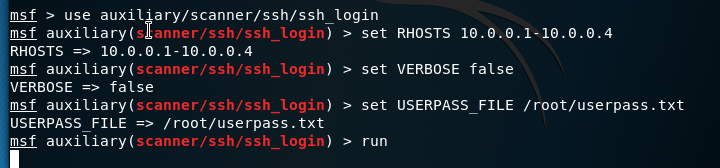
\includegraphics[width=0.70\linewidth]{figures/comandos}}
\caption{Comandos utilizados para o ataque de força bruta}
\small{Fonte - (próprio autor, 2018)}
\label{Fig:Comandos utilizados para o ataque de força bruta}
\end{center} \end{figure}

O primeiro comando "set RHOSTS 10.0.0.1-10.0.0.4", corresponde aos endereços para testar os usuários e senhas, ou seja, são as vítimas. O comando "set VERBOSE false". Quer dizer que só deve imprimir as tentativas que deu certo. O comando "set USERPASS\_FILE /root/userpass.txt", significa o caminho que está a \textit{wordlist}. Após a utilização destes comandos, o \textit{framework} testa todas as possibilidades inseridas no arquivo userpass.txt. Se o usuário e a senha corresponder a qualquer vítima, são exibidos a senha e o username, como ilustrado na figura \ref{Fig:Resultados do ataque de força bruta}.

\begin{figure}[htbp!] \begin{center}
% fbox faz uma borda ao redor do seu argumento
\fbox{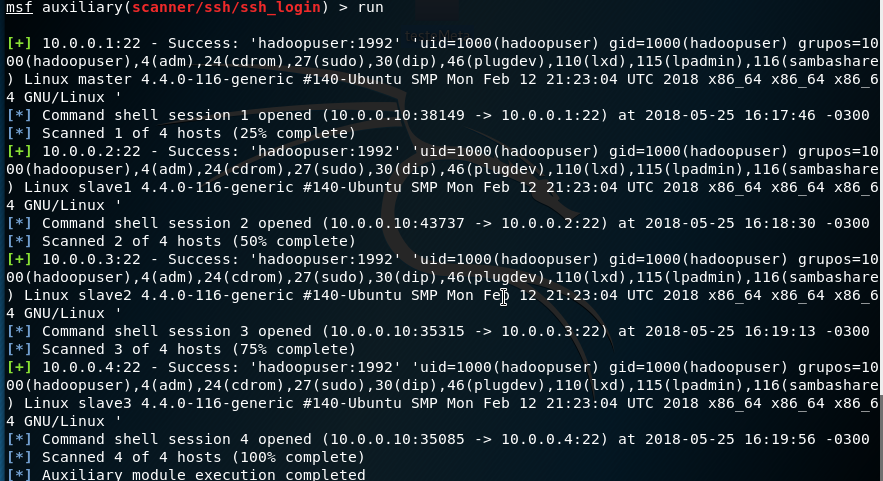
\includegraphics[width=0.80\linewidth]{figures/resultadoDoMetasploit}}
\caption{Resultados do ataque de força bruta}
\small{Fonte - (próprio autor, 2018)}
\label{Fig:Resultados do ataque de força bruta}
\end{center} \end{figure}

De acordo com os resultados obtidos na figura \ref{Fig:Resultados do ataque de força bruta}, percebe-se que ao tentar força bruta nos hosts com a faixa de IP 10.0.0.1 até 10.0.0.4, que é justamente o cluster, foram encontrados os usuários e as senhas dos mesmos. Percebe-se que o usuário do host 10.0.0.1 é 'hadoopuser' e a senha é '1992', para o restante dos hosts é a mesma senha e o mesmo usuário. Em posse desses dados é possível ter acesso via ssh aos nós do cluster ou até mesmo ao nó \textit{master} pela máquina atacante, como demonstrado na figura \ref{Fig:AcessoClusterPeloKali}.  Nela é demonstrado que do terminal do kali linux que é a máquina atacante, especificamente do terminal do metasploit, foi possível acessar o cluster.


\begin{figure}[htbp!] \begin{center}
% fbox faz uma borda ao redor do seu argumento
\fbox{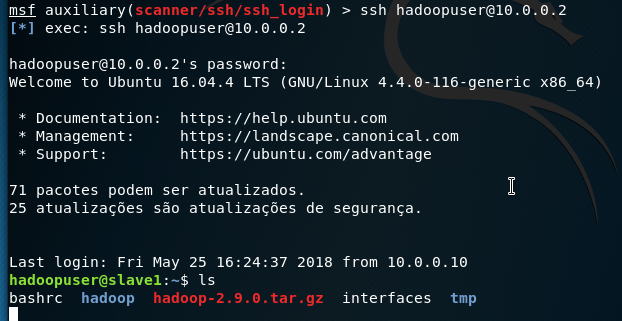
\includegraphics[width=0.80\linewidth]{figures/testandoUserPassword}}
\caption{Acessando o cluster pelo terminal do atacante}
\small{Fonte - (próprio autor, 2018)}
\label{Fig:AcessoClusterPeloKali}
\end{center} \end{figure}

Deve-se levar em consideração que esse ataque está em um ambiente controlado e que foi realizada uma engenharia social no proprietário para obter informações pessoais e com isso poder gerar uma \textit{wordlist} para tentar descobrir a senha e o usuário do cluster. Porém, obter informações de pessoas nos dias de hoje, não é uma tarefa muito difícil, tendo em vista que as redes sociais, sites de cadastros e outros meios na internet fornecem muitas informações nos quais os atacantes podem ter acesso de forma fácil e com isso poder fazer várias combinações e gerar arquivos com terabytes de senhas possíveis e tentar um ataque de força bruta. Conseguindo fazer isso e tendo acesso a um cluster ou até mesmo a uma aplicação o atacante pode usar sua imaginação e levar sérios prejuízos aos proprietários e as empresas.

\subsubsection{Boas práticas de segurança}

Em muitas configurações de e-mails, senhas de banco, senhas em geral, elas têm relação com o usuário ou com a empresa, estão relacionadas de alguma forma, seja por data de nascimento, por dia comemorativo, time de futebol, música, filmes, e entre outras relações que podem ser feitas para se gerar um dicionário e conseguir fazer uma força bruta para descobrir usuários e senhas.

Então, sabendo disso para o segundo cenário, as boas práticas de segurança consistem em senha fortes, contendo nomes minúsculos, maiúsculos, caracteres especiais e números, sem contar que ela deve ser grande no sentido de extensão, ou seja, uma senha com no mínimo quinze caracteres combinando os caracteres já citados. Isso dificulta um ataque de força bruta, e não ser relacionada com a empresa, ou seja, não deve conter nenhum nome ou qualquer caractere que se relacione com a empresa. 

Além das senhas fortes, uma outra prática importante seria limitar o acesso pelo ssh somente via chave pública realizando a configuração no OpenSSH, no caminho /etc/ssh/ssh\_config, para isso bastaria mudar para "no" as cláusulas PasswordAuthentication e UsePAM, além de gerar o par de chaves para os usuários e equipamentos envolvidos na autenticação (clientes e servidores). Habilitando o ssh para utilizar somente chaves públicas e privadas, há uma necessidade de proteger a privacidade dessas chaves, colocando-as em uma pasta na qual apenas o usuário root tenha acesso.

Essas práticas de senhas fortes e alterar a configuração do ssh são pouco praticadas entre empresas, pois no dia a dia os gestores necessitam rapidez e eficiência, não se preocupam com a segurança. Isso preocupa não só pela facilidade de descobrir as senhas ou burlar o sistema como também no uso de uma engenharia social efetuada pelo atacante para poder obter outros dados.

\newpage
\section{Cenário III}
Neste cenário a ideia principal consiste em realizar um ataque \textit{man in the middle} , ou seja, ficar no meio da comunicação entre os nós do cluster e conseguir executar tarefas, tais como: iniciar o nó, parar o nó, ter controle, logo, para o nó atacado a máquina atacante será o seu \textit{master}. Como explicado anteriormente, o ataque consiste em poluir a tabela ARP de um host e fazer com que ele se reporte ao atacante pensando que é o host verídico.

Para este ataque foram utilizadas algumas ferramentas, tais como: Ettercap, ubuntu 16.04, wireshark e foi necessário instalar o \textit{framework} Apache Hadoop nesta nova máquina atacante. A ideia inicial era instalar o Hadoop no sistema operacional Kali Linux, porém ao realizar os precedimentos de instalação houve diversos erros, alguns que poderiam comprometer os outros testes, com isso, optou-se por instalar o Ettercap e o wireshark em uma máquina Ubuntu, e realizar o ataque a partir dela, onde pra isso foi necessário colocar ela na rede, como ilustra a figura \ref{Fig:novoAmbiente}.

\begin{figure}[htbp!] \begin{center}
% fbox faz uma borda ao redor do seu argumento
\fbox{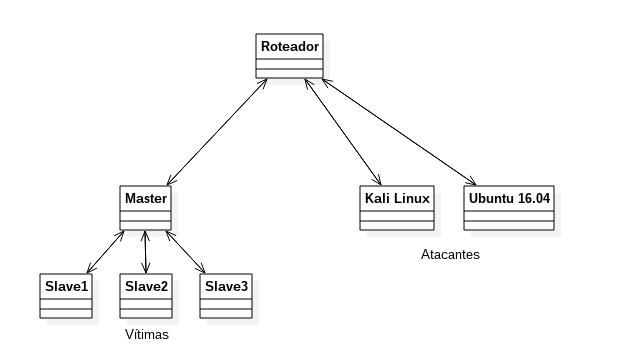
\includegraphics[width=0.80\linewidth]{figures/novoCenario}}
\caption{Visão geral do novo ambiente}
\small{Fonte - (próprio autor, 2018)}
\label{Fig:novoAmbiente}
\end{center} \end{figure}

Após isso, o ataque foi executado na seguinte ordem: Primeiro foi iniciado o nmap, para saber quais os hosts estão disponíveis na rede, com isso, foi obtido o resultado que ilustra a figura \ref{Fig:Scaneado a rede com nmap}. Selecionando a vítima, o próximo passo é iniciar o Ettercap, pois com ele será possível executar o arp-spoofing, que consiste em poluir a tabela ARP da vítima. A figura \ref{Fig:Interface do Ettercap} ilustra a interface da ferramenta, nela o primeiro passo é clicar em 'Sniff' e selecionar o modo 'Unified sniffing', após isso irá aparecer um \textit{PopUp} pedindo pra escolher a placa de rede, após isso basta ir na aba 'Hosts' e clicar em 'Scan for hosts' em seguida na mesma aba clica em 'Host List', depois desses passos serão listados os hosts da rede scaneada, com isso basta selecionar o host que será a vítima, clicar em target, ir na aba 'MITM' e selecionar a opção 'ARP poisoning', depois disso é só clicar em 'Start' que o ataque começa.

\begin{figure}[htbp!] \begin{center}
% fbox faz uma borda ao redor do seu argumento
\fbox{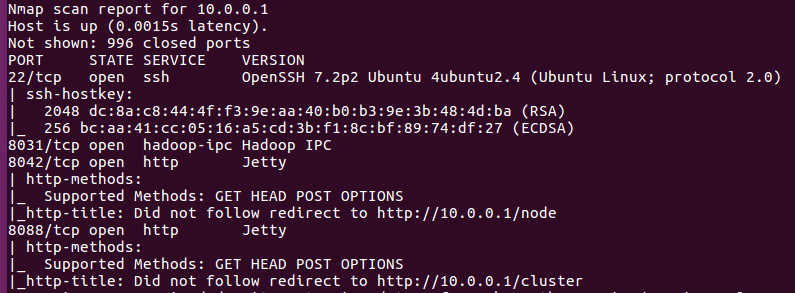
\includegraphics[width=0.80\linewidth]{figures/nmapNovoCenario}}
\caption{Scaneado a rede com nmap}
\small{Fonte - (próprio autor, 2018)}
\label{Fig:Scaneado a rede com nmap}
\end{center} \end{figure}

%%%%%%%%%%%%%%%%%%%%%%%%%%%%%%%%%%%%%%%%%%%%%%%%%%%%%%%%%%%%%%%

\begin{figure}[htbp!] \begin{center}
% fbox faz uma borda ao redor do seu argumento
\fbox{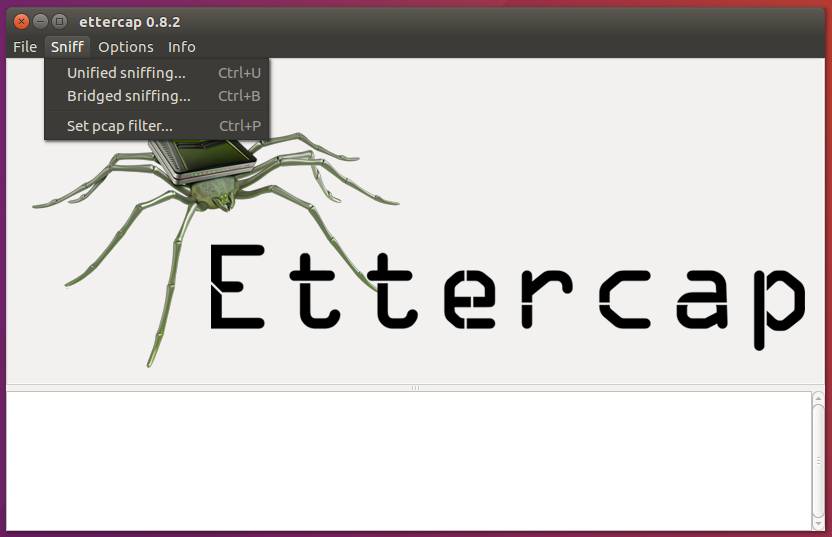
\includegraphics[width=0.80\linewidth]{figures/ettercap01}}
\caption{Interface do Ettercap}
\small{Fonte - (próprio autor, 2018)}
\label{Fig:Interface do Ettercap}
\end{center} \end{figure}

%AQUI É PRA EXPLICAR MAIS SOBRE A TABELA ARP

Como explicado anteriormente, esse ataque consiste em poluir a tabela ARP da vítima, ou seja, na tabela ARP contém todos os dados associados aos endereços IP e MAC, então ao realizar o envio dos dados do atacante para a tabela ARP da vítima ocorre a poluição da tabela, confundindo a vítima para que ela se comunique com o atacante pensando que está se comunicando com o \textit{master}, pois esse ataque foi direcionado a um nó do cluster, a vítima escolhida foi o \textit{slave1} com o endereço de IP 10.0.0.2. Para saber se o ataque está funcionando, o Hadoop foi iniciado no \textit{master}. Com isso, ao abrir o \textit{slave1} e digitar o comando "arp -a" ou "arp -n" pois esse comando serve para dizer qual o endereço MAC e IP o \textit{slave} está se comunicando. A figura \ref{Fig:Comando arp -n antes do ataque} ilustra o comando "arp -n" no \textit{slave1} antes do ataque, e a figura \ref{Fig:Comando arp -n durante o ataque} ilustra o comando "arp -n" no \textit{slave1} durante a execução do ataque \textit{man in the middle}.
%duas imagens aqui para fazer a visualização
%
\begin{figure}[htbp!] \begin{center}
% fbox faz uma borda ao redor do seu argumento
\fbox{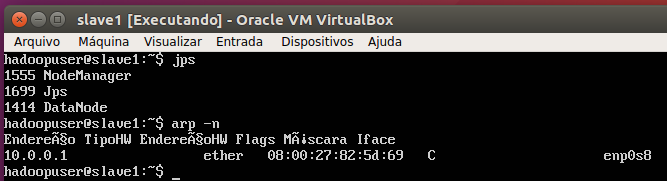
\includegraphics[width=0.90\linewidth]{figures/comandoarpAntesdoAtaque}}
\caption{Comando arp -n antes do ataque}
\small{Fonte - (próprio autor, 2018)}
\label{Fig:Comando arp -n antes do ataque}
\end{center} \end{figure}


\begin{figure}[htbp!] \begin{center}
% fbox faz uma borda ao redor do seu argumento
\fbox{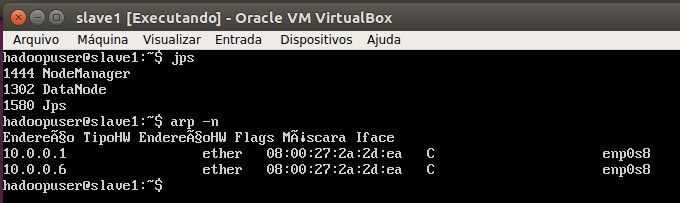
\includegraphics[width=0.90\linewidth]{figures/comandosDepoisAtaque}}
\caption{Comando arp -n durante o ataque}
\small{Fonte - (próprio autor, 2018)}
\label{Fig:Comando arp -n durante o ataque}
\end{center} \end{figure}


Como ilustram as figuras \ref{Fig:Comando arp -n antes do ataque} e \ref{Fig:Comando arp -n durante o ataque} ocorreu uma alteração no endereço MAC do nó \textit{master}, ou seja, o endereço MAC do nó \textit{master} passou a ser o endereço MAC do atacante como ilustra a figura \ref{Fig:Comando arp -n durante o ataque}. Com isso, o \textit{slave1} quando for se comunicar com o \textit{master} ele estará se comunicando com o atacante, pois o endereço MAC do atacante está associado ao IP do \textit{master}.

Para saber se o ataque está mesmo funcionando, ou seja, se o \textit{slave1} está mesmo se comunicando com o atacante ao invés de está se comunicando com o \textit{master}, basta acessar o atacante e tentar parar o nó \textit{slave1}, como ilustra a figura \ref{Fig:Stop Slave1}


\begin{figure}[htbp!] \begin{center}
% fbox faz uma borda ao redor do seu argumento
\fbox{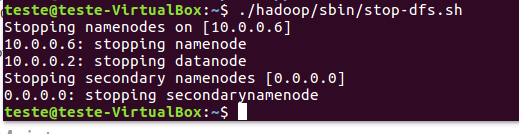
\includegraphics[width=0.90\linewidth]{figures/stopingSlave1}}
\caption{Stop Slave1}
\small{Fonte - (próprio autor, 2018)}
\label{Fig:Stop Slave1}
\end{center} \end{figure}

Como ilustra a figura \ref{Fig:Stop Slave1} percebe-se que o datanode com o IP 10.0.0.2 está stopping, ou seja, ele é parando, esse IP é justamente o IP do \textit{Slave1}, além disso ao acessar o \textit{Slave1} e verificar se está funcionando alguma aplicação percebe-se ao executar o comando jps, apenas duas aplicações estão funcionando, ao invés de três aplicações, como ilustra a figura \ref{Fig:Atividades Slave1 depois do Stop}.

\begin{figure}[htbp!] \begin{center}
% fbox faz uma borda ao redor do seu argumento
\fbox{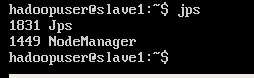
\includegraphics[width=0.72\linewidth]{figures/depoisDoStopPeloAtacante}}
\caption{Atividades Slave1 depois do Stop}
\small{Fonte - (próprio autor, 2018)}
\label{Fig:Atividades Slave1 depois do Stop}
\end{center} \end{figure}

Ao acessar o painel do Apache Hadoop e verificar a situação dos datanodes, percebe-se que o \textit{Slave1} não está funcionando, ou seja, o atacante conseguiu parar o datanode e com isso o ataque foi realizado com sucesso, como ilustra a figura \ref{Fig:painelDatanodeStop}.

\begin{figure}[htbp!] \begin{center}
% fbox faz uma borda ao redor do seu argumento
\fbox{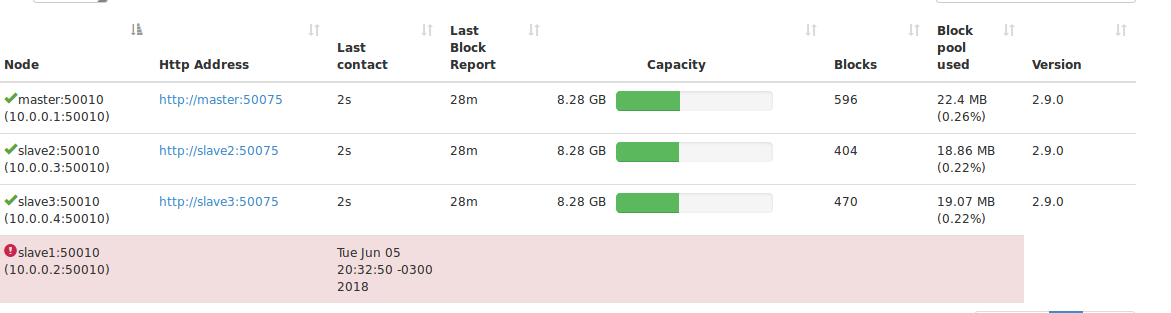
\includegraphics[width=0.90\linewidth]{figures/painelDatanodeStop}}
\caption{Painel Datanode Stop}
\small{Fonte - (próprio autor, 2018)}
\label{Fig:painelDatanodeStop}
\end{center} \end{figure}

Vale salientar que o atacante estava de posse das chaves do ssh para que o ataque funcionasse com perfeição, pois sem elas não seria possível ocorrer a comunicação entre a máquina atacante e o slave1. Sem as chaves do ssh, apenas era possível poliur a tabela ARP da vítima, mas não seria possível realizar o stop no DataNode.


Sendo assim, o \textit{man in the middle} foi realizado com sucesso, considerando que esse ataque está em um ambiente controlado, ele não dará nenhuma dor de cabeça, porém, se esse ataque fosse em larga escala, em um ambiente de produção? Seria uma dor de cabeça enorme para os desenvolvedores, sem contar que a empresa seria atingida.

\subsubsection{Boas práticas de segurança}

Durante um ataque \textit{man in the middle}, o host do atacante distribui seu próprio endereço MAC juntamente com seu endereço de IP em \textit{broadcast}, fazendo com que a vítima insira esses dados na sua tabela ARP. Visto isso, as boas práticas de segurança utilizadas neste cenário consistem em utilizar um Sniffer de pacotes na rede procurando as mensagens ARP que estão sendo enviadas aleatoriamente, ou seja, em \textit{broadcast}.

Uma outra maneira de se defender de um ataque MITM seria utilizando um IP estático, ou seja, fixar o IP e o endereço MAC do roteador na tabela ARP da vítima, pois quando o atacante enviasse seus dados IP e MAC em broadcast, querendo se passar pelo roteador, não iria funcionar, pois na tabela ARP da vítima já consta o IP e o MAC associados a outro host.

As chaves do ssh são de fundamental importância para que se possa ter acesso ao cluster, sendo assim, torna-se imprescindível que essas chaves sejam protegidas em uma pasta criptografada ou somente ao alcance do usuário root. Pois, em caso de não proteção corre-se o risco de comprometer todo o funcionamento do cluster.

O MITM é um ataque utilizado de várias formas, ele pode ser utilizado para roubar dados dos usuários através dos navegadores, capturar informações através da comunicação entre hosts e neste cenánio ele foi utlizado para ter acesso a um nó do cluster poluindo a tabela ARP da vítima. Sendo assim, para cada caso existem suas peculiaridades, porém, de forma geral uma maneira de identificar esse ataque é implantando um sniffer na rede ou sendo precavido e adicionando o IP e o MAC do roteador diretamente na tabela ARP da máquina utilizada.


%%%%%%%%%%%%%%%%%%%%%%%%%%%%%%%%%%%%%%%%%%%%%%%%%%%%%%%%%%%%%%
